\chapter{Local structure of LSCO+O}\label{ch:local}
In this chapter, we look at structural correlations in La$_{2-x}$Sr$_x$CuO$_{4+\delta}$ (LSCO+O) containing oxygen interstitials. As discussed in section \ref{sec:lscoo}, LSCO+O is known to form complex superstructures that shows up in single-crystal diffraction. To quickly recap, `staging' \cite{Wells1997,Ray2017} was discovered early on and appears unrelated to superconductivity. On the other hand, novel superstructures, known as `Local Lattice Distortions' (LLD) and `Oxygen Interstitials' (O$_\text{i}$), are suggested to have a connection with superconductivity \cite{Poccia2011}. In fact, it appears that these two orderings are anti-correlated in real space, forming `puddles' on \SI{}{\micro\meter} scale \cite{Poccia2012}.

The data shown in this chapter is a collection of experiments performed on three different instruments: IN8, ThALES and D4 at Institut Laue-Langevin\todo{what is the best way to cite the instruments?} in Grenoble, France. In the first part, we explore some of the superstructures mentioned above in two single crystals of LSCO+O: La$_2$CuO$_{4+\delta}$ ($T_\text{c} = \SI{43}{\kelvin}$) and La$_{1.94}$Sr$_{0.06}$CuO$_{4+\delta}$ ($T_\text{c} = \SI{37.5}{\kelvin}$). In the second part, we perform a diffraction experiment on powders of LSCO+O with the purpose of looking at real space correlation through pair-distribution-function (PDF) analysis.

\section{Superstructures in single crystals}\label{sec:single_crystal_superstructures}
While superstructures in LSCO+O have been extensively studied in the past, it is always useful to check if your samples comply with previous observations. The measurements shown here were mostly performed as a reference for some of the work shown in chapter \ref{ch:lowen}, but I present it here since it has relevance for structural correlations and can help us with the analysis of the PDF data in the following section. Superstructures in LCO+O are generally observed at $Q_2 = (0, 0.21, 0.29)$ and $Q_3 = (0.09, 0.24, 0.50)$ \cite{Kusmartsev2000} and should thus mainly be observable in the $a$-$c$ (or equivalently $b$-$c$ due to twinning\todo{mention twinning in introduction}) plane.

When using certain Triple-Axis spectrometers (IN8, IN20, ThALES) at the ILL, we have the option of a secondary spectrometer (everything after the sample) called FlatCone \cite{flatcone} where we can probe a large part of reciprocal space simultaneously. In particular, the FlatCone analyser system is built in such a way that you probe a large part of the scattering plane at a constant energy transfer $\hbar\omega$. In the following we are interested in structural correlations, so we are measuring at $\hbar\omega = 0$. In chapter \ref{ch:lowen} we will investigate finite energy transfers in detail.

\begin{figure}
    \centering
    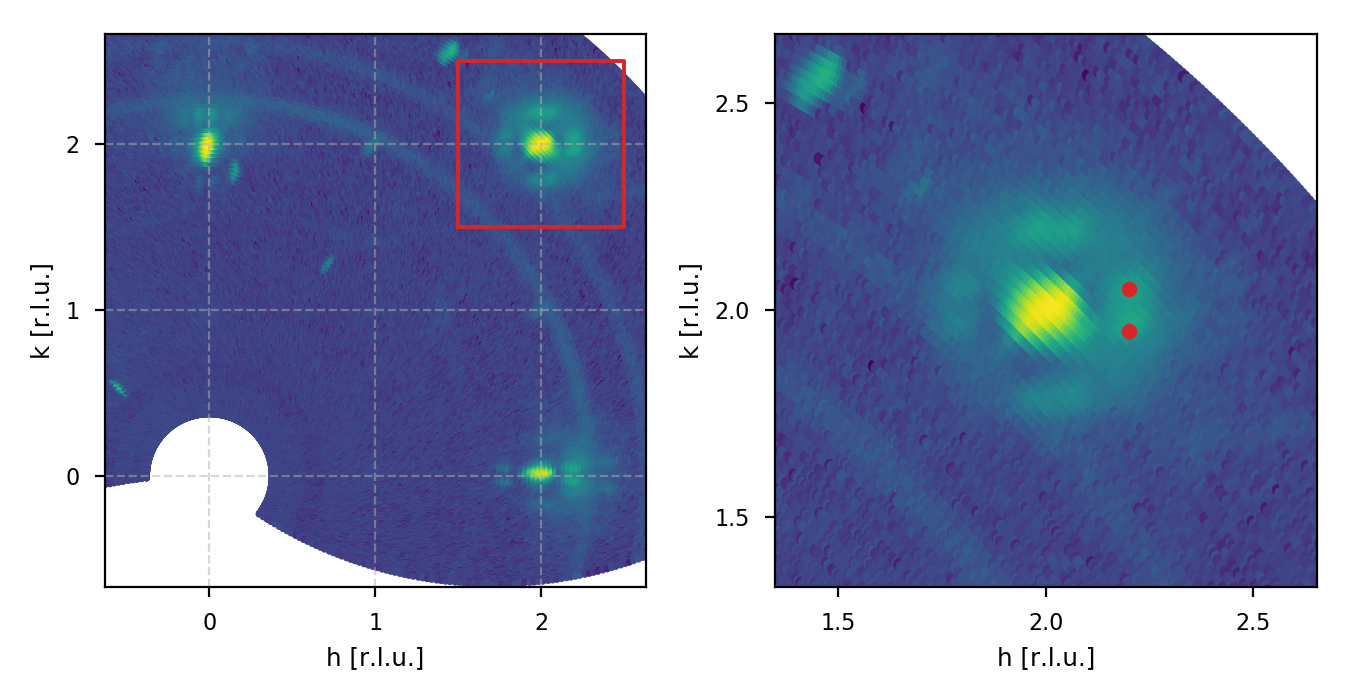
\includegraphics[width=0.9\textwidth]{fig/pdf/lcoo_ab_elastic.png}
    \caption{Reciprocal space map of single crystal La$_2$CuO$_{4+\delta}$, measured in the $a$-$b$ plane with the unconventional Bmab orthorhombic coordinate system. \textbf{Left}: Full map, showing mainly the fundamental Bragg peaks. Circular arcs are powder lines from Al. \textbf{Right}: Zoomed-in view of the are marked in red. We notice satellite peaks around (220) at $Q=(0.2,\pm 0.05,0)$ ($|Q| = \SI{0.241}{\per\angstrom}$).}
    \label{fig:lcoo_ab_elastic}
\end{figure}

Figure \ref{fig:lcoo_ab_elastic} shows the result of such a measurement of La$_2$CuO$_{4+\delta}$ on the thermal TAS IN8, performed in the $a$-$b$ plane using the orthorhombic coordinate system (see section \ref{sec:lscoo} in chapter \ref{ch:intro}\todo{maybe put a dedicated section in the introduction or simulation chapter}). The coverage of our measurement is such that we see the (200), (020) and (220) fundamental Bragg peaks.Some satellite peaks are visible at roughly $Q = (0.2, \pm 0.05, 0)$ as marked on the zoomed-in right-hand-side of the figure. Satellite peaks with zero $l$-component has been previously observed by our group \cite{Ray2016}, but the nature of these peaks are currently unknown. We can, however, make the simple observation that this peak corresponds to a real-space structural correlation with a length $d_1 \approx \SI{26}{\angstrom}$ in the $a-b$ plane.

\begin{figure}
    \centering
    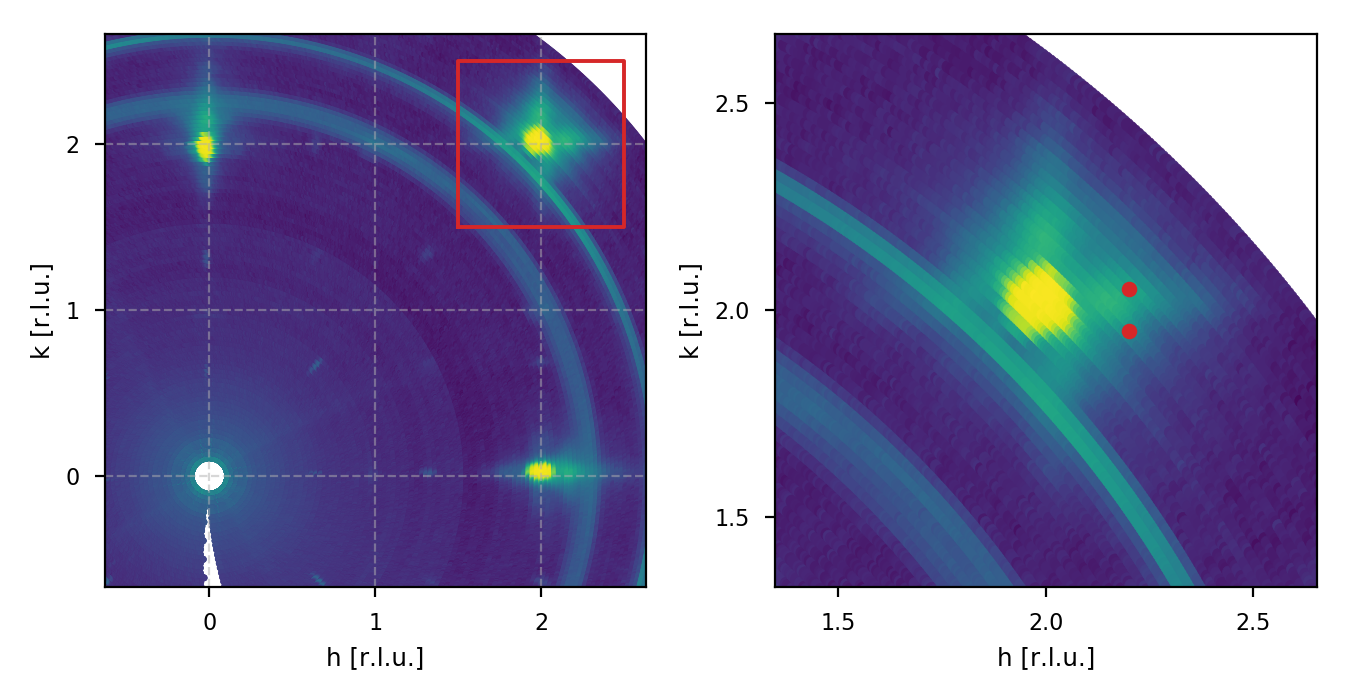
\includegraphics[width=0.9\textwidth]{fig/pdf/lscoo_ab_elastic.png}
    \caption{Reciprocal space map of single crystal La$_{1.94}$Sr$_{0.06}$CuO$_{4+\delta}$, measured in the $a$-$b$ plane with the unconventional Bmab orthorhombic coordinate system. \textbf{Left}: Full map, showing mainly the fundamental Bragg peaks. Circular arcs are powder lines from Al. \textbf{Right}: Zoomed-in view of the are marked in red, showing diffuse scattering. The marks are at identical locations to figure \ref{fig:lcoo_ab_elastic} as a reference for comparison.}
    \label{fig:lscoo_ab_elastic}
\end{figure}

Figure \ref{fig:lscoo_ab_elastic} shows the same type of measurement, but this time of La$_{1.94}$Sr$_{0.06}$CuO$_{4+\delta}$ on the cold TAS ThALES. While similar features are visible, the satellites seen in figure \ref{fig:lcoo_ab_elastic} are smeared out, suggesting that the tiny amount of Sr in this sample causes a significant amount of disorder which shows up as diffuse satellites.

\begin{figure}
    \centering
    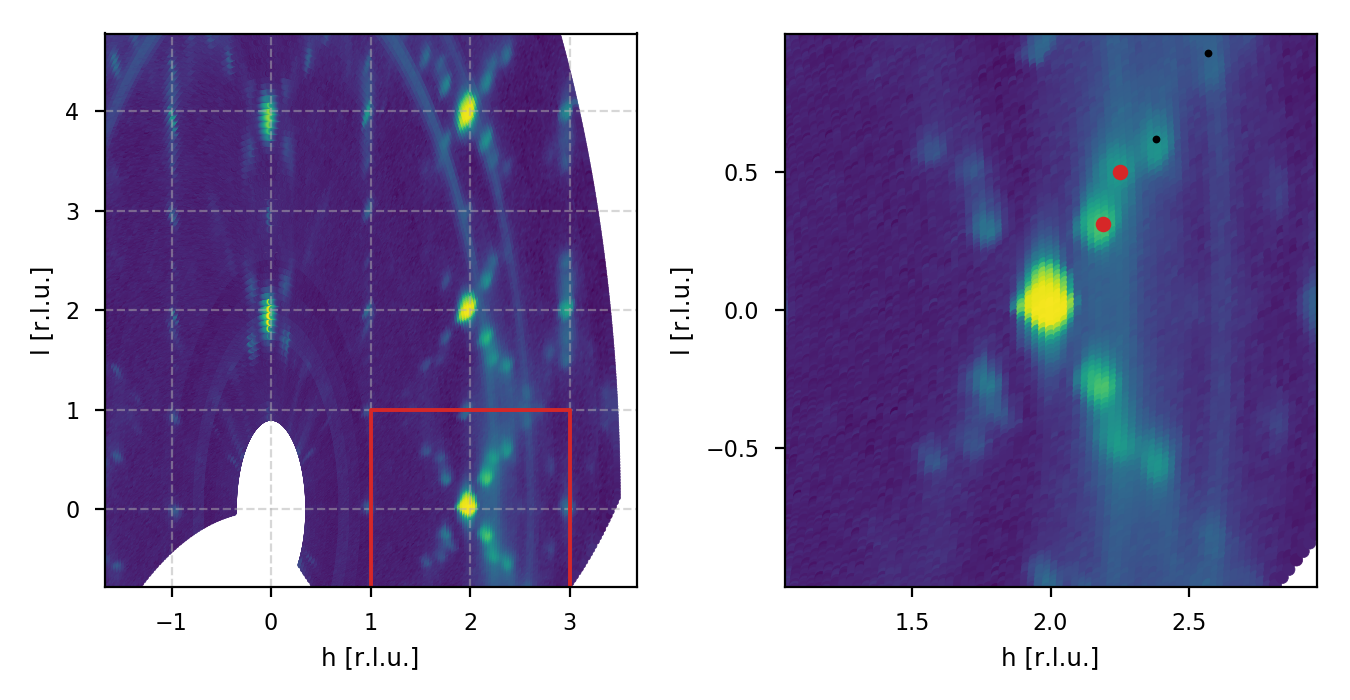
\includegraphics[width=0.9\textwidth]{fig/pdf/lscoo_ac_elastic.png}
    \caption{Reciprocal space map of single crystal La$_2$CuO$_{4+\delta}$, measured in the $a$-$c$ plane with the unconventional Bmab orthorhombic coordinate system. \textbf{Left}: Full map, showing mainly the fundamental Bragg peaks. Circular arcs are powder lines from Al. \textbf{Right}: Zoomed-in view of the are marked in red. We notice satellite peaks around (002) at $Q_2=(0.19,0,0.31)$ ($|Q_2| = \SI{0.267}{\per\angstrom}$) and $Q_3=(0.25,0,0.5)$ ($|Q_3| = \SI{0.378}{\per\angstrom}$).}
    \label{fig:lscoo_ac_elastic}
\end{figure}

Finally, in figure \ref{fig:lscoo_ac_elastic}, we show a measurement of La$_2$CuO$_{4+\delta}$ in the $a$-$c$ plane performed on ThALES. This measurement is entirely consistent with superstructures known from literature \cite{Kusmartsev2000}, and we can clearly index the peaks as $Q_2 = (0.19, 0, 0.31)$ (even showing \nth{2} and \nth{3} order reflections) and $Q_3 = (0.25,0,0.5)$. The correlation lengths associated with these peaks are $d_2 \approx \SI{24}{\angstrom}$ and $d_3 \approx \SI{17}{\angstrom}$, respectively.

While none of these measurements are new (see \cite[Chapter 10]{Ray2016}), they help to confirm that the samples we use for spectroscopic measurements in chapters \ref{ch:lowen}, \ref{ch:anomaly}, \ref{ch:arpes} are comparable to previous samples. In addition, I believe it highlights an unsolved problem with regards to figuring out exactly what the nature of these structural correlations are and what (if any) relationship they have with superconductivity.

While constructing models for these superstructures is outside the scope of this thesis, they help identify some general length scales that might be relevant in a real-space model. Unfortunately, we also immediately notice that these correlations are inaccessible in our DFT MD simulations from chapter \ref{ch:md}, where the maximal simulation box is a $2 \times 2 \times 1$ cell such that the only non-zero $\bm{Q}$ we can represent is $(\frac{1}{2}\frac{1}{2}{0})$. These length scales, while rather large, are still accessible by PDF measurements as we shall see below.

\section{Real-space correlation in powders}
We now turn to experiments performed on a series of powdered samples, where we use an instrument well-suited for obtaining \emph{real-space} correlations (see section \ref{sec:specific_neutron}, chapter \ref{ch:method}) using the pair-distribution function (PDF). There are multiple purposes to this experiment. 

First, we want to simply measure oxygen-doped La$_{2-x}$Sr$_x$CuO$_{4+\delta}$ with the PDF method. From single-crystal measurements, as we saw above, it is well known that the presence of oxygen interstitials result in intricate long-range ordering phenomena. This ordering is, to my knowledge, usually not detectable in diffraction experiments on powders, but we were motivated by the fact that diffraction experiments optimized for PDF analysis are well-suited for determining correlations at \SIrange{5}{25}{\angstrom}.

Second, we wanted to see if oxygen ordering we could detect oxygen re-ordering caused by cooling rate. Single crystal measurements have shown that certain structural peaks can be removed by `quenching', that is, rapid cooling from \SIrange{300}{200}{\kelvin} in single crystal samples of La$_2$CuO$_{4+\delta}$ \cite{Poccia2012}.

\begin{figure}
    \centering
    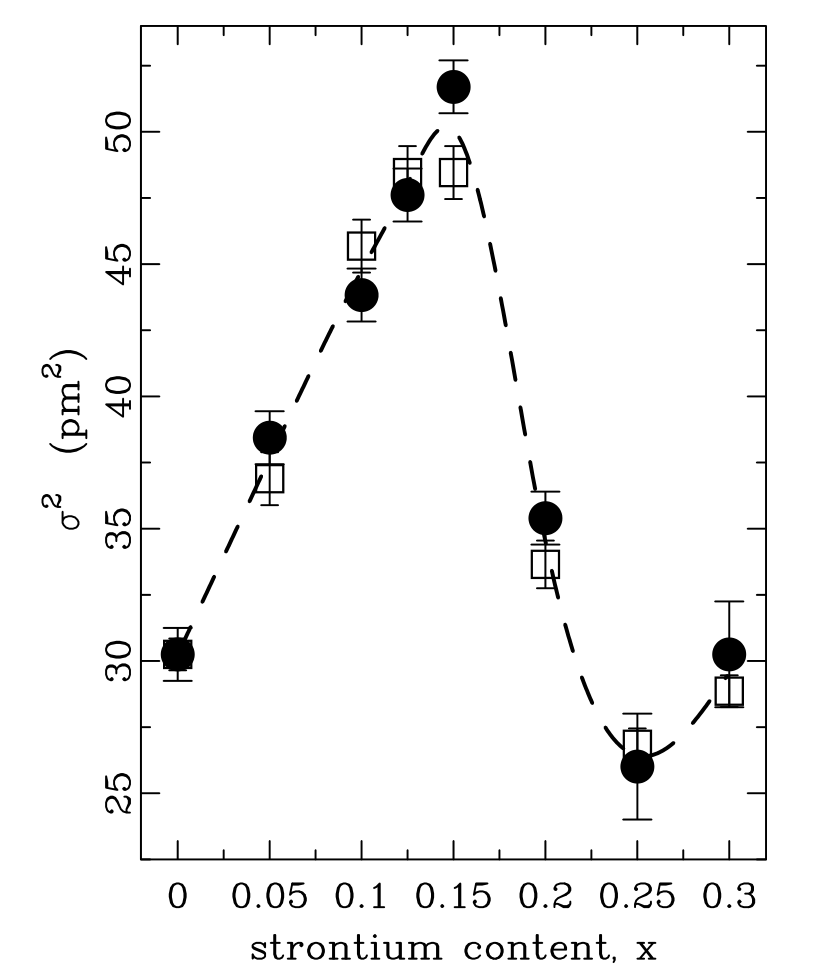
\includegraphics[width=0.4\textwidth]{fig/pdf/bozin_cuo.png}
    \caption{Relationship between strontium content $x$ in La$_{2-x}$Sr$_x$CuO$_4$ (LSCO) and the width of the Cu-O equatorial bond distribution $\sigma$. For reference, LSCO is superconducting from $x=0.05$ to $x=0.25$ and reaches the largest $T_\text{c}$ at $x=0.15$. Figure from \cite{Bozin2000}}
    \label{fig:bozin_cuo}
\end{figure}

Third, PDF measurements of La$_{2-x}$Sr$_x$CuO$_4$ have shown that the \emph{distribution} of Cu-O distances is heavily influenced by doping \cite{Bozin2000}. In addition, the distribution is widest at optimal $T_\text{c}$ as shown in figure \ref{fig:bozin_cuo}. Since we are using a completely different dopant species, it is interesting to ask this same question for our samples. Finally, we want to compare high and low temperature phases to look for any peculiarities related to superconductivity or other low-temperature phases.

\subsection{Samples}
Three powdered samples were measured:

\begin{itemize}
    \item \textbf{LCO}: La$_2$CuO$_4$ (\SI{2.7844}{\gram}, insulating)
    \item \textbf{LCO+O}: La$_2$CuO$_{4.05}$ (\SI{0.7403}{\gram}, $T_\text{c} \approx \SI{40}{\kelvin}$)
    \item \textbf{LSCO3+O}: La$_{1.97}$Sr$_{0.03}$CuO$_{4.05}$ (\SI{3.3612}{\gram}, $T_\text{c} \approx \SI{40}{\kelvin}$)
\end{itemize}

\noindent Measurements were performed at the Disordered materials diffractometer D4 at Institut Laue-Langevin in Grenoble, France. Reduction and transformation of data was performed at the instrument with software specifically built for D4. All steps of the data treatment is saved, but we will mainly use the fully reduced and normalized datasets in both $Q$- and $r$-space. When comparing subtle differences between spectra (such as the same sample after different cooling procedures), we might construct a difference curve from the raw data since the background subtractions will cancel out.

\subsection{Experiment}
Table \ref{tab:measurments} contains a list of the measurements performed in the order which they were performed. The quenching was performed by submerging the \SI{300}{\kelvin} sample in liquid nitrogen and then transferring to the \SI{100}{\kelvin} cryostat. Annealing was performed by heating the cryostat to \SI{350}{\kelvin} for about an hour which is known to disorder the oxygen \cite{Poccia2012}. The reason we performed the quenching before the annealing was due to time constraints. Each acquisition was approximately 2 hours.

\begin{table}
    \centering
    \begin{tabular}{llll}
        \toprule
        index &   sample & temperature &      state \\
        \midrule
        0  &      LCO &         300 &    initial \\
        1  &    LCO+O &         300 &    initial \\
        2  &    LCO+O &         100 &   quenched \\
        3  &    LCO+O &          15 &   quenched \\
        4  &    LCO+O &         300 &   quenched \\
        5  &    LCO+O &         350 &  annealing \\
        6  &    LCO+O &         300 &   annealed \\
        7  &    LCO+O &         100 &   annealed \\
        8  &    LCO+O &          15 &   annealed \\
        9  &    LCO+O &         300 &   annealed \\
        10 &  LSCO3+O &         300 &    initial \\
        11 &  LSCO3+O &         100 &   quenched \\
        12 &  LSCO3+O &          15 &   quenched \\
        13 &  LSCO3+O &         350 &  annealing \\
        14 &  LSCO3+O &          15 &   annealed \\
        \bottomrule
    \end{tabular}
    \caption{List of measurements performed at D4 in chronological order. `Quenched' refers to the rapid cooling as described in the text, and annealing refers to keeping the sample at \SI{350}{\kelvin} for roughly 30 minutes.}
    \label{tab:measurments}
\end{table}

In summary we have a total of three samples to compare at \SI{300}{\kelvin}. For the oxygen-doped samples we can additionally look at the low temperature phase as well as the difference between `quenched' and `annealed' doping.

\subsection{Results}
We start with the second objective of figuring out if there is any difference due to cooling procedure. Figure \ref{fig:difference} shows the difference between cooling procedures for the two oxygen-doped samples. In general there are no systematic differences apart from the slight decline of the difference curve for the LCO+O sample. This is likely due to a small amount of hydrogen in the cryostat as a consequence of the quenching procedure. The preliminary conclusion is that there is no difference between quenched and annealed measurements to a high degree of certainty. This is somewhat surprising since it is well known that certain structural peaks can be removed from quenching in single crystals \cite{Poccia2012}. We cannot conclude if our result is due to the sample being a powder or due to rotational averaging. Since we detect no difference in the spectra, we can use the annealed \SI{15}{\kelvin} data and initial \SI{300}{\kelvin} data for the remaining analysis.


\begin{figure}
    \centering
    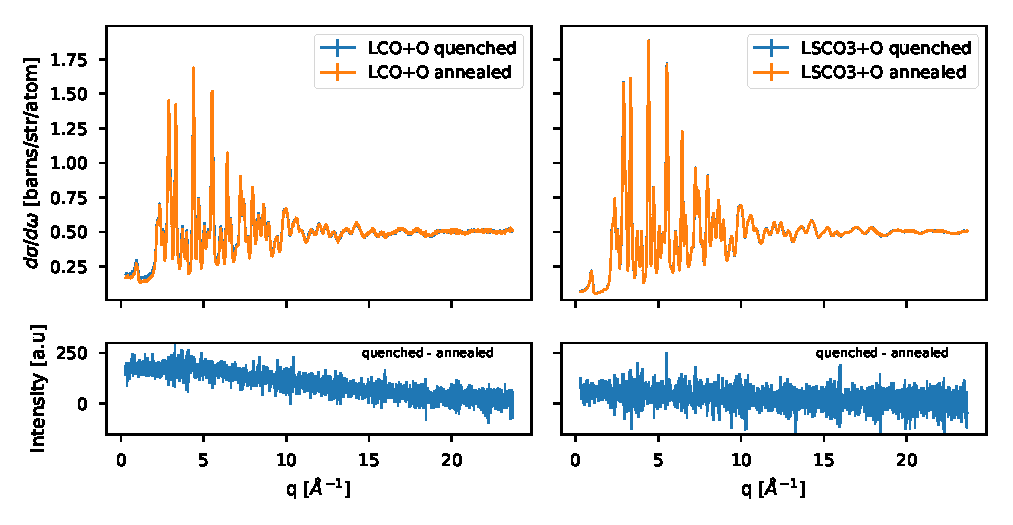
\includegraphics[width=\textwidth]{fig/pdf/quenched_annealed.pdf}
    \caption{Difference between quenched and annealed cooling procedures for LCO+O and LSCO3+O samples. The topmost plots are comparisons of the reduced and corrected $\text{d}\sigma/\text{d}\omega$ in absolute units, while the difference curves are extracted from the raw $\bm{q}$ data.}
    \label{fig:difference}
\end{figure}

In Figure \ref{fig:sample_comparision} we compare the three samples at \SI{300}{\kelvin} in both real and reciprocal space. While the differences are quite small, the difference curves (green) seem to be larger between parent/oxygenated compounds compared to the two oxygenated compounds. This is consistent with a picture where oxygen distorts the lattice in a meaningful way, while the effect of a small amount of strontium is negligible. Figure \ref{fig:temperature_comparision} shows the high- and low-temperature data for the two oxygen-doped samples. At first glance there seems to be nothing out of the ordinary, peaks are shifting slightly due to thermal expansion (this is particularly easy to spot in the real-space data).

\begin{figure}
    \centering
    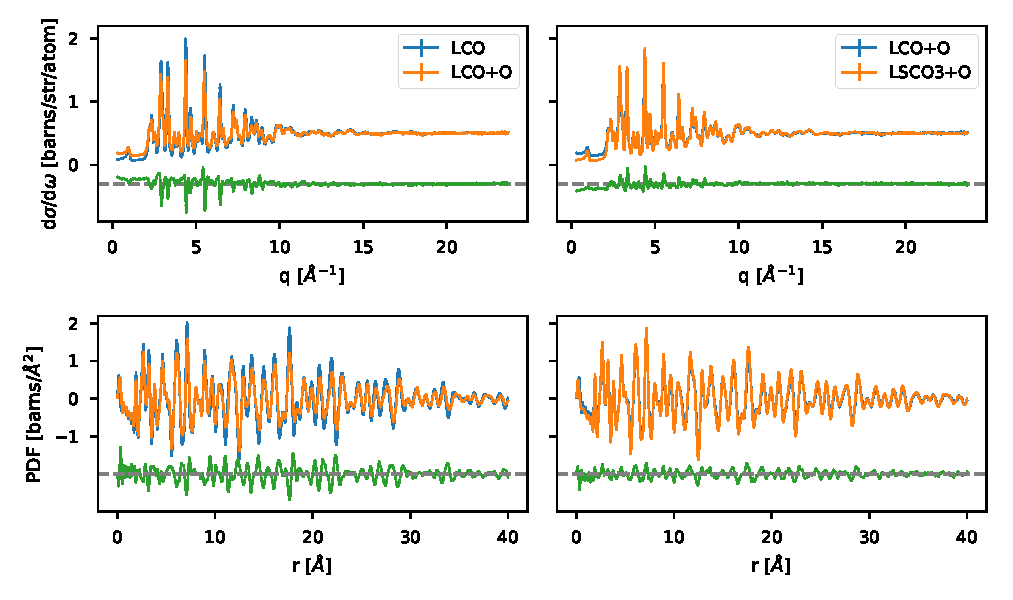
\includegraphics[width=\textwidth]{fig/pdf/sample_comparison.pdf}
    \caption{Comparison of the three different samples at \SI{300}{\kelvin} in both real and reciprocal space. On the \textbf{left} we compare LCO with LCO+O in order to see if there is an effect of oxygen. On the \textbf{right} we look at LCO+O versus LSCO3+O to have a similar comparison between two \emph{different} oxygen-doped samples.}
    \label{fig:sample_comparision}    
\end{figure}

\begin{figure}
    \centering
    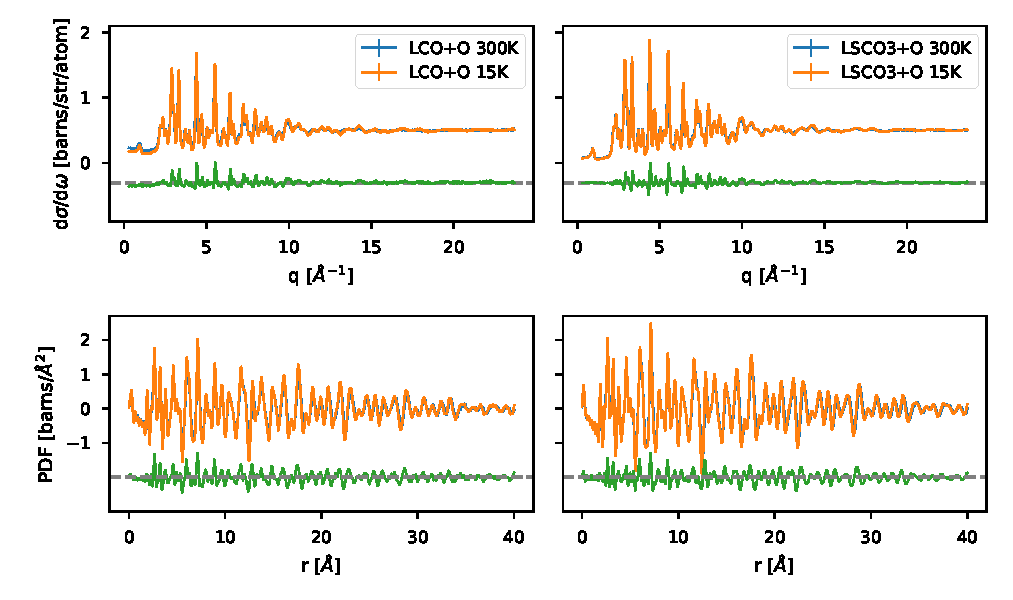
\includegraphics[width=\textwidth]{fig/pdf/temperature_comparison.pdf}
    \caption{Temperature dependence of \SI{300}{\kelvin} and \SI{15}{\kelvin} for LCO+O and LSCO3+O in both real and reciprocal space.}
    \label{fig:temperature_comparision}    
\end{figure}

\subsection{Analysis}
Without performing detailed modelling, we can take a look at the first peak in the real-space data which corresponds to the Cu-O in-plane bond. This bond-length is suspected to be important for superconductivity by controlling the Coulomb interaction (the Hubbard-$U$) \cite{Ivashko2019}. Previously, as mentioned above, measurements on La$_{2-x}$Sr$_x$CuO$_{4}$ have shown that the width of the Cu-O bond-length distribution is largest at optimal doping $x=0.15$ and qualitatively tracks the superconducting dome \cite{Bozin2000}. We fit the first peak of all relevant datasets to a single Gaussian as shown in Figure \ref{fig:cu_o_fits} and report the fitting parameters in Table \ref{tab:cu_o_fits}.

\begin{figure}
    \centering
    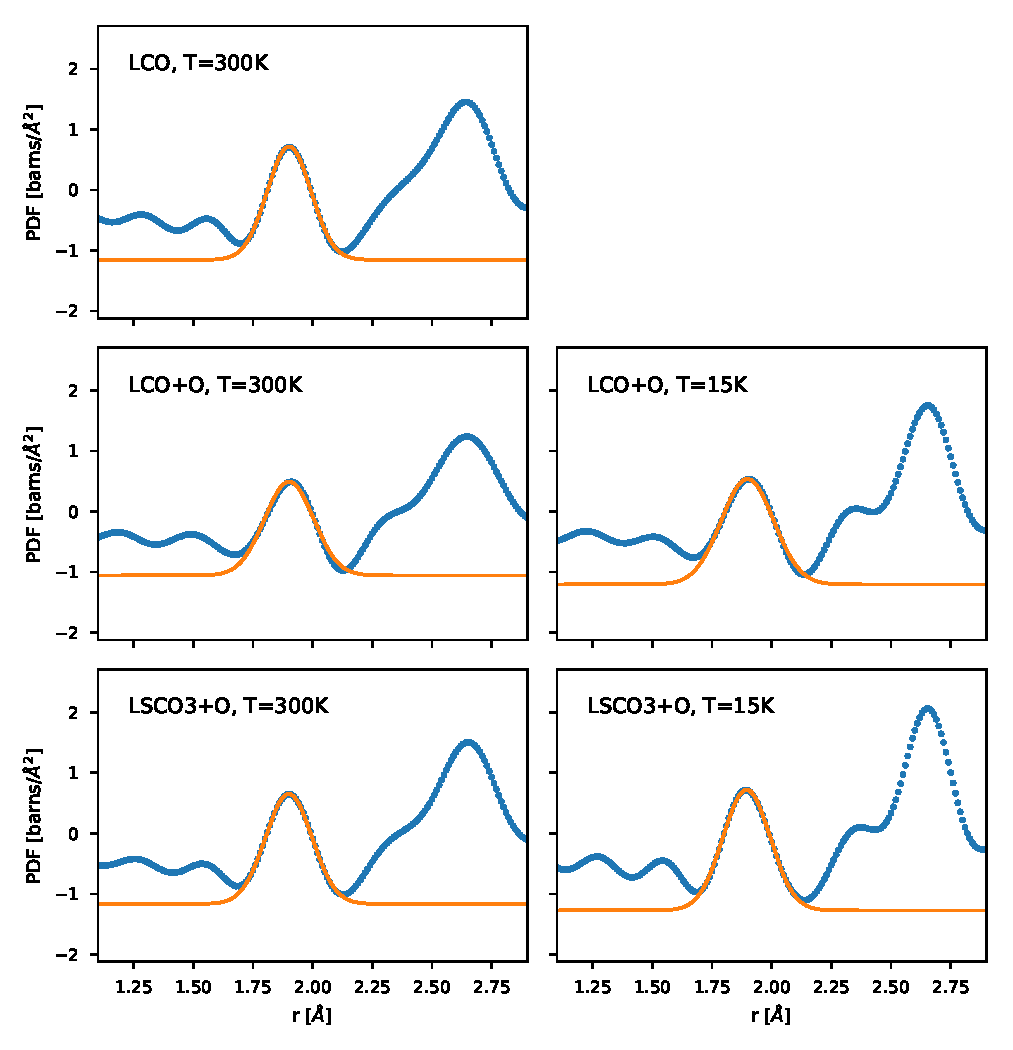
\includegraphics[width=\textwidth]{fig/pdf/cu_o_fits.pdf}
    \caption{Cu-O distance Gaussian fits. For each of the five temperature/sample combinations (figure text), the short range PDF is shown along with a Gaussian fit of the first peak. In order to compare between the fits, the constant background has been fixed to $-1.2$}
    \label{fig:cu_o_fits}
\end{figure}

\begin{table}
    \centering
    \begin{tabular}{llll}
        \toprule
          Sample & Temperature [K] &   Cu-O mean distance &           Cu-O sigma \\
        \midrule
             LCO &             300 &  1.9010 $\pm$ 0.0003 &  0.0941 $\pm$ 0.0003 \\
           LCO+O &             300 &  1.9005 $\pm$ 0.0012 &  0.1112 $\pm$ 0.0014 \\
         LSCO3+O &             300 &  1.8995 $\pm$ 0.0003 &  0.0989 $\pm$ 0.0004 \\
           LCO+O &              15 &  1.8983 $\pm$ 0.0009 &  0.1096 $\pm$ 0.0010 \\
         LSCO3+O &              15 &  1.8944 $\pm$ 0.0003 &  0.0951 $\pm$ 0.0004 \\
        \bottomrule
    \end{tabular}
    \caption{Cu-O distances in all samples at all available temperatures as extracted from the fits in figure \ref{fig:cu_o_fits}.}
    \label{tab:cu_o_fits}
\end{table}

Comparing to La$_{2-x}$Sr$_x$CuO$_{4}$, we have roughly the same peak position at $r=\SI{1.9}{\angstrom}$. At \SI{300}{\kelvin} LCO has a smaller width compared to LCO+O and LSCO3+O. At \SI{15}{\kelvin} the widths are slightly smaller as one would expect from the reduced temperatures. Our measurements are thus consistent with the observations of \cite{Bozin2000}, that the Cu-O bond-length tracks $T_c$ , but with an entirely different dopant species. Interestingly, the sample with a small amount of Sr has a slightly smaller $\sigma$.

\begin{figure}
    \centering
    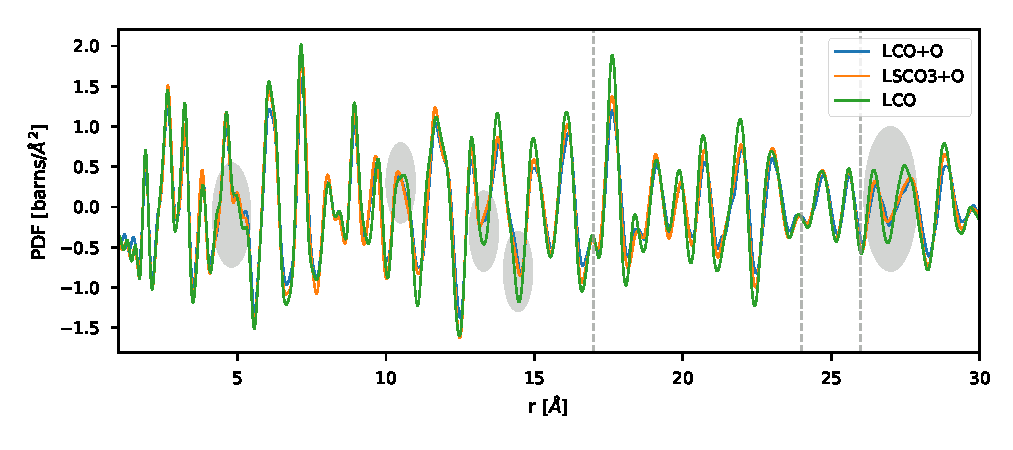
\includegraphics[width=\textwidth]{fig/pdf/300k_all.pdf}
    \caption{PDF at \SI{300}{\kelvin} for the three samples studied here across the accessible range. Differences between stoichiometric and oxygen-doped samples are highlighted with grey circles. Grey vertical lines mark the correlation lengths identified in section \ref{sec:single_crystal_superstructures}.}
    \label{fig:pdf_all_300K}
\end{figure}

In figure \ref{fig:pdf_all_300K}, we take a closer look at the PDF from the three samples obtained at \SI{300}{\kelvin}. As we mentioned earlier, any differences between the plots are quite subtle, but our initial analysis that there is a `larger' difference between LCO and LCO+O when compared to the difference between LCO+O and LSCO3+O seems to be correct. Marked in figure \ref{fig:pdf_all_300K} are regions where there is a qualitative difference between the curves. That is, we don't just see sharpening/broadening, but the shape of the peaks are noticeably different. In addition, I marked the possible correlation lengths identified in the previous section.

Unfortunately, there seems to be no real signature of a change due to interstitial that is related to the superstructures identified earlier. In addition, even though there are differences where we can clearly separate the oxygen-doped samples from La$_2$CuO$_4$, the changes that we do see are barely noticeable.

Finally, in figure \ref{fig:pdf_sim_comparision} I compare LCO and LCO+O at \SI{300}{\kelvin} with molecular dynamics simulations in the LTO phase also at \SI{300}{\kelvin} on an absolute scale. In general, we seem to have a quite good agreement between experiment and simulation, especially with regards to the short range correlations around \SI{3}{\angstrom}. Noticeably, the shortest Cu-O bond is significantly sharper in the simulation, so perhaps we are not accurately describing short range forces. At higher $r$, the simulation PDF naturally dies out due to limited system size.

\begin{figure}
    \centering
    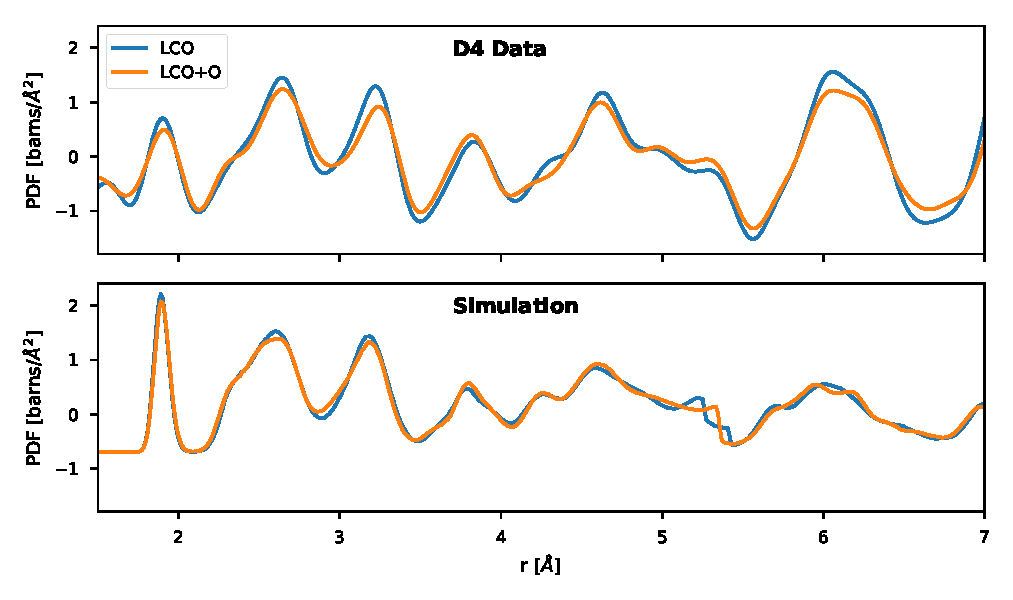
\includegraphics[width=\textwidth]{fig/pdf/pdf_simulation_experiment_compare.pdf}
    \caption[PDF data compared with MD simulation]{PDF data compared with MD simulation}
    \label{fig:pdf_sim_comparision}
\end{figure}

\section{Summary}
In this chapter, we performed experiments with the intention of gaining a further understanding of the various superstructures present in LSCO+O. Through single-crystal measurements we independently confirmed the existence of the superstructures reported by various groups \cite{Kusmartsev2000} and additionally observed in-plane satellites only seen by us \cite{Ray2016}.

We performed high-quality PDF measurements of 3 powdered samples with and without interstitial oxygen, confirming subtle differences due to interstitials. A direct connection to the superstructures observed in single crystals could, however, not be made. If this is a consequence of superstructures not being visible in the rotationally averaged diffraction pattern or if the powders are different with regards to superstructure signatures, is hard to say. Our measurements appears consistent with the observation of \citeauthor{Bozin2000} \cite{Bozin2000} and have an increased distribution of in-plane Cu-O distances in superconducting samples, slightly more so in LCO+O compared to LSCO3+O.

Finally, the MD simulations performed in chapter \ref{ch:md} are consistent with the shape of the measured PDF, especially in the \SIrange{2}{4}{\angstrom} range. In order to properly describe the differences we see at higher correlation lengths, some real space modelling and/or reverse monte-carlo fitting of the PDF would be required to properly analyse the data. The work performed in this chapter could thus be used as a first step for constructing real-space models of non-stoichiometric oxides.

